\begin{table*}[t]
\centering\small
\caption{Expanded offline benchmark: final accuracy (\%) $\pm$ sample standard deviation over ten paired seeds. Central budgets are 40 for Digits and 200 for Fashion-MNIST and CIFAR-10. Anchors have different storage budgets.}
\label{tab:offlineexpanded}
\begin{tabular}{lrrr}\toprule
Selector & Digits & Fashion-MNIST & CIFAR-10\\\midrule
Random & 89.47 $\pm$ 1.96 & 75.11 $\pm$ 4.43 & 39.13 $\pm$ 0.83 \\
Balanced random & 89.61 $\pm$ 2.31 & 76.32 $\pm$ 2.85 & 38.92 $\pm$ 1.19 \\
Doubt & 89.61 $\pm$ 4.65 & 56.29 $\pm$ 7.22 & 35.25 $\pm$ 9.02 \\
Curiosity & 89.16 $\pm$ 4.03 & 53.16 $\pm$ 3.52 & 38.36 $\pm$ 1.47 \\
EgoGate & 89.50 $\pm$ 4.75 & 52.41 $\pm$ 3.51 & 38.09 $\pm$ 1.82 \\
Embedding k-center & 88.94 $\pm$ 2.23 & 64.18 $\pm$ 4.53 & 38.50 $\pm$ 1.50 \\
EgoGate-diverse & 91.78 $\pm$ 2.55 & 56.08 $\pm$ 3.85 & 38.21 $\pm$ 1.36 \\
High loss & 89.97 $\pm$ 4.55 & 49.86 $\pm$ 2.40 & 38.45 $\pm$ 1.31 \\
Herding adaptation & 90.62 $\pm$ 2.05 & 76.94 $\pm$ 3.05 & 39.35 $\pm$ 1.09 \\
No replay & 49.53 $\pm$ 0.32 & 48.38 $\pm$ 3.48 & 35.32 $\pm$ 8.95 \\
Full-pool replay & 95.91 $\pm$ 1.15 & 80.32 $\pm$ 2.24 & 52.25 $\pm$ 3.35 \\
\bottomrule\end{tabular}
\end{table*}

\begin{table}[t]\centering\small
\caption{EgoGate minus random storage in final accuracy (percentage points), with pointwise seed-paired 95\% intervals and Holm-adjusted $p$ values from the 27-test primary family.}
\label{tab:offlinecontrasts}
\begin{tabular}{lrrr}\toprule
Dataset / $K$ & Difference & 95\% CI & $p_{\mathrm{Holm}}$\\\midrule
Digits / 20 & -5.58 & [-7.61, -3.55] & 0.003 \\
Digits / 40 & +0.03 & [-3.43, +3.50] & 1.000 \\
Digits / 100 & +1.56 & [-0.33, +3.46] & 1.000 \\
Fashion / 50 & -17.23 & [-20.77, -13.69] & $<0.001$ \\
Fashion / 200 & -22.70 & [-25.76, -19.64] & $<0.001$ \\
Fashion / 500 & -24.24 & [-26.45, -22.03] & $<0.001$ \\
CIFAR-10 / 50 & -0.45 & [-1.12, +0.22] & 1.000 \\
CIFAR-10 / 200 & -1.04 & [-2.02, -0.06] & 0.561 \\
CIFAR-10 / 500 & -3.51 & [-4.85, -2.16] & 0.004 \\
\bottomrule\end{tabular}
\end{table}

\begin{figure*}[t]
\centering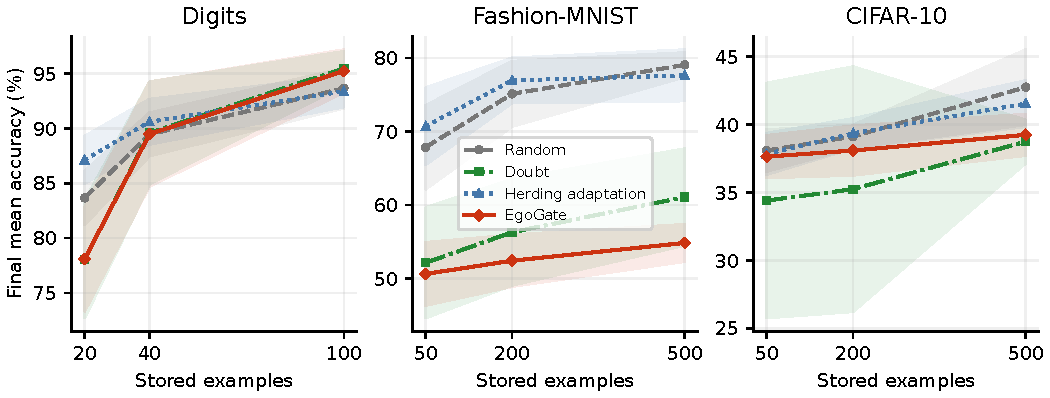
\includegraphics[width=\textwidth]{offline_benchmark.pdf}
\caption{Expanded offline benchmark across storage budgets. Lines show ten-seed means; shading shows one sample standard deviation, not a confidence interval. Primary significance tests use paired differences and Holm correction.}
\label{fig:expanded}
\end{figure*}

\subsection{Completed GPU Results}
All 870 runs completed on two Tesla T4 GPUs: 810 bounded-selector runs and
60 anchors. The audit verifies the complete grid, unique observations, matched
update/exposure counts, and selected-index hashes. Execution used Python
3.13.16, PyTorch 2.11.0+cu130, torchvision 0.26.0+cu130, CUDA 13.0,
NumPy 2.1.3, SciPy 1.16.3, and scikit-learn 1.6.1.

The expanded study does not establish a general advantage for EgoGate.
Across nine dataset/budget cells it has no significant wins over random,
Doubt, or herding after correction across the 27 primary tests. It has five
significant losses against random and five against herding: Digits at $K=20$,
all three Fashion-MNIST budgets, and CIFAR-10 at $K=500$. No comparison with
Doubt rejects after correction. Non-rejection is not evidence of equivalence.

At the central budgets (Table~\ref{tab:offlineexpanded}), Digits final accuracy
is 89.50\% for EgoGate and 89.47\% for random. Their paired difference is
$+0.03$ points, with a 95\% interval of $[-3.43,3.50]$. This differs from the
original fixed-split retention result. Randomized class partitions, data splits,
separated random generators, and the final-accuracy endpoint all change the
evaluation; the experiment does not isolate which change explains the discrepancy.

On Fashion-MNIST at $K=200$, EgoGate reaches 52.41\%, versus 75.11\% for
random and 76.94\% for herding. The EgoGate--random difference is $-22.70$
points (95\% interval $[-25.76,-19.64]$, Holm $p=1.02\times10^{-6}$).
Old-task accuracy is 15.92\% for EgoGate and 61.06\% for random, while
new-task accuracy is 88.90\% and 89.17\%, respectively. Thus the deficit
primarily concerns retention rather than a gain in new-task learning. EgoGate
still covers an average 4.9 of five old classes; counting represented classes
alone is insufficient to explain or prevent this failure.

CIFAR-10 exposes a severe limitation of the entire low-replay regime. At
$K=200$, random and EgoGate retain only 3.54\% and 1.73\% old-task accuracy,
despite 80.19\% mean accuracy before Task B. New-task accuracies are 74.72\%
and 74.45\%. Their final means, 39.13\% and 38.09\%, therefore conceal
near-complete old-task failure. The full-pool anchor reaches 52.25\% final
accuracy, which also falls short of strong continual learning. These results
must not be presented as competitive CIFAR performance or a comprehensive
comparison of modern continual-learning systems.

\subsection{Cost and Interpretation}
At CIFAR-10 $K=200$, mean EgoGate selection costs 10.48 s, versus less than
0.001 s for random and 0.88 s for herding. Task-B training takes about 25.3 s
for each. These synchronized timings exclude loading, base training, and final
evaluation; they quantify this implementation on the recorded hardware, not
universal latency. Equal update counts do not imply equal total compute.

The memory curves (Fig.~\ref{fig:expanded}) and complete secondary results
are supplied alongside all primary contrasts. A descriptive high mean for
EgoGate-diverse on Digits is not a confirmed primary-comparison win. Increasing
storage does not guarantee that global difficulty ranking becomes representative.
The study strengthens the evidence about the limits of the original selector;
it does not rescue its general-superiority claim. More replay, stronger
architectures, tuned optimization, and complete published baselines remain
necessary before drawing conclusions about broader continual-learning methods.
